\section[Lineaaristen yhtälöryhmien sovellusesimerkkejä]{*Lineaaristen yhtälöryhmien 
perinteisiä \\ sovellusesimerkkejä} 
\label{yhtälöryhmät} 
\sectionmark{Perinteiset lineaariset yhtälöryhmät}
\alku

Tietokoneiden avulla suoritettavalle laajamittaiselle tieteellis-tekniselle laskennalle 
--- esimerkiksi numeeriselle sään ennustamiselle --- on tyypillistä, että huomattava osa 
tietokoneen käyttämästä laskenta-ajasta kuluu suurten lineaaristen yhtälöryhmien ratkaisuun. 
Yhtälöryhmiin päädytään, kun tarkastelun kohteena olevat luonnonlait (säätä ennustettaessa 
virtausmekaniikan perusyhtälöt) \kor{diskretoidaan}, eli muunnetaan numeerisen laskennan 
kannalta soveliaaseen likimääräiseen muotoon. Laskemisen palauttaminen nimenomaan
\pain{lineaarisiksi} yhtälöryhmiksi on malleissa tavallista senkin vuoksi, että lähinnä
vain tämän tyyppisten perustehtävien numeerisen ratkaisemisen tietokone viime kädessä 'osaa'.

Modernien tieteellis-teknisten laskentatehtävien ohella suuren lineaarisen yhtälöryhmän ongelma
on keskeinen myös monissa perinteisemmissä --- usein tietokonetta paljon vanhemmissa --- 
matemaattisissa malleissa, joita esiintyy erityisesti insinööritieteissä. Seuraavassa esitetään
kaksi tällaista klassista sovellusesimerkkiä, toinen sähkötekniikasta ja toinen rakenteiden 
mekaniikasta.

\subsection*{Sähköpiiri: Vastusverkko}
\index{zza@\sov!Szyhkzzc@Sähköpiiri: Vastusverkko|vahv}

\begin{multicols}{2}
\parbox{2in}{Tarkastellaan klassista sähköpiiriä, joka on pelkkien \pain{vastusten} muodostama
verkko. Olkoot verkon solmupisteet $P_i,\ i = 1 \ldots n$, ja olkoot pisteet $P_i,\,P_j$ 
yhdistetty vastuksella $R_{ij}$ (jollei suoraa yhteyttä ole, asetetaan $1/R_{ij}\,=\,0$
yhtälöryhmässä \eqref{m-8.3} jäljempänä). Oheisessa kuvassa on yleinen neljän solmun verkko.}
\begin{figure}[H]
\begin{center}
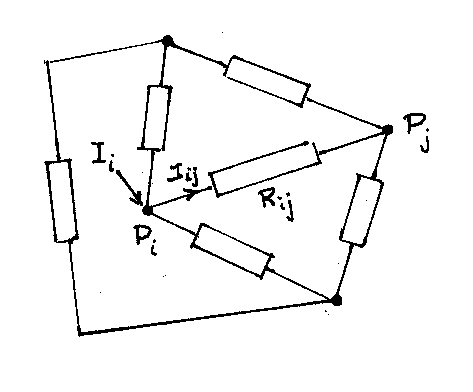
\epsfig{file=kuvat/kuvaM-1.ps}
\end{center}
\end{figure}
\end{multicols}
Jos merkitään $I_{ij} =$ \pain{virta} vastuksen $R_{ij}$ läpi, positiivisena $P_i$:stä poispäin
(vrt.\ kuvio), niin 
\index{Kirchhoffin laki}%
\pain{Kirchhoffin} \pain{lain} (\hist{G.R. Kirchhoff}, 1845) mukaan
\begin{equation} \label{m-8.1}
\sum_{j=1}^n I_{ij}\ =\ I_i, \quad i = 1 \ldots n,
\end{equation}
missä $I_i =$ solmuun $P_i$ ulkoapäin syötetty virta. Toisaalta
\index{Ohmin laki}%
\pain{Ohmin} \pain{lain} (\hist{G.S. Ohm}, 1826) mukaan
\begin{equation} \label{m-8.2}
R_{ij} I_{ij}\ =\ V_i - V_j, \quad i,j = 1 \ldots n,
\end{equation}
missä $V_i =$ j\pain{ännite} solmussa $P_i$. Ohmin lakia \eqref{m-8.2} käyttäen voidaan virrat
$I_{ij}$ yhtälöryhmässä \eqref{m-8.1} lausua jännitteiden avulla, jolloin tuloksena on systeemi
\begin{equation} \label{m-8.3}
\sum_{j=1}^n a_{ij} V_j\ =\ I_i, \quad i = 1 \ldots n,
\end{equation}
missä
\[
a_{ii}\ =\ \sum_{j=1}^n (1/R_{ij}), \quad a_{ij}\ =\ -1/R_{ij},\,\ i \neq j.
\]
Tämä on lineaarinen yhtälöryhmä kokoa $n \times n$, missä $x_i = V_i$, $b_i = I_i$. 
\begin{Exa} Jos nelisolmuisessa verkossa (vrt.\ kuvio edellä) on 
$R_{ij} = R,\ i,j = 1 \ldots 4,\ i \neq j$, niin jännitteille
$V_i$ saadaan yhtälöryhmä
\[ \left\{ \begin{array}{rrrrrrrrl} 3V_1&-& V_2&-& V_3&-& V_4&\ \ =\ \ &RI_1\\
                                    -V_1&+&3V_2&-& V_3&-& V_4&\ \ =\ \ &RI_2\\
                                    -V_1&-& V_2&+&3V_3&-& V_4&\ \ =\ \ &RI_3\\
                                    -V_1&-& V_2&-& V_3&+&3V_4&\ \ =\ \ &RI_4
\end{array} \right. \]
Tämä on singulaarinen systeemi: Jos esim.\ $I_1 = I \neq 0$ ja $I_2 = I_3 = I_4 = 0$, niin 
ratkaisua ei ole. Jos myös $I_1 = 0$, niin $V_i = V,\ i = 1 \ldots 4$ on ratkaisu millä tahansa
$V \in \R$, ts.\ ratkaisuja on äärettömän monta. \loppu 
\end{Exa}
 
Esimerkin singulaarisuusongelma on yhtälöryhmän \eqref{m-8.3} ominaisuus yleisemminkin.
Nimittän kertoimien $a_{ij}$ ym.\ lausekkeista nähdään, että
\[
\sum_{j=1}^n a_{kj}\ =\ \sum_{i=1}^n a_{ik}\ =\ 0, \quad k = 1 \ldots n.
\]
Tästä on kaksi seuraamusta: Ensinnäkin jos yhtälöryhmän \eqref{m-8.3} yhtälöt lasketaan 
puolittain yhteen saadaan
\[
(\sum_{i=1}^n a_{i1})\,V_1 + \ldots + (\sum_{i=1}^n a_{in})\,V_n\ =\ \sum_{i=1}^n I_i,
\]
eli
\begin{equation} \label{m-8.4}
0\ =\ \sum_{i=1}^n I_i.
\end{equation}
Toiseksi nähdään, että jos $\seq{V_i}$ on systeemin \eqref{m-8.4} ratkaisu, niin myös 
$\seq{V_i + V}$ on ratkaisu millä tahansa $V \in \R$, sillä
\[
\sum_{j=1}^n a_{ij} (V_j + V)\ =\ \sum_{j=1}^n a_{ij} V_j\ +\ (\sum_{j=1}^n a_{ij})\,V\ 
                               =\ I_i + 0\ =\ I_i, \quad i = 1 \ldots n.
\]
On siis päätelty: (a) Jos yhtälöryhmällä \eqref{m-8.3} on ratkaisu, niin ehto \eqref{m-8.4} 
toteutuu, ts.\ tämä on \pain{välttämätön} \pain{ehto} ratkeavuudelle. (b) Jos yhtälöryhmä 
\eqref{m-8.3} on ratkeava, niin ratkaisuja on äärettömän monta. Yhtälöryhmä \eqref{m-8.3} on 
siis yleisesti singulaarinen.

Singulaarisuusongelma on merkki siitä, että matemaattista mallia ei ole ajateltu 
(fysikaaliselta kannalta) aivan loppuun asti. --- Ongelmaan onkin yksinkertainen 
'sähkömiehen ratkaisu': \pain{Maadoitetaan} verkon yksi solmu $P_k$. Matemaattisessa mallissa
tämä merkitsee solmussa $P_k$ asetettavia ehtoja
\begin{equation} \label{m-8.5}
V_k\ =\ V_{ref}, \quad I_k\ =\ - \sum_{i \neq k} I_i.
\end{equation}
Ensimmäinen ehto asettaa jännitteelle $V_k$ jonkin valinnaisen referenssiarvon $V_{ref}$, esim.\
$V_{ref} = 0$. Tämä on luvallista, koska fysikaalisesti merkitseviä ovat vain jännite-erot. 
Toisessa ehdossa voidaan $I_k$ tulkita \pain{maadoitusvirraksi}, joka määräytyy fysikaalisesti
siten, että syöttövirtojen tasapainoehto \eqref{m-8.4} (myös fysikaalinen ehto!) toteutuu. Ehto
$V_k = V_{ref}$ poistaa $V_k$:n tuntemattomien joukosta, jolloin yhtälöryhmä \eqref{m-8.3} 
voidaan kirjoittaa muotoon
\[
\sum_{j \neq k} a_{ij} V_j\ =\ I_i - a_{ik} V_{ref}\ = J_i, \quad i = 1 \ldots n.
\]
Tästä voidaan edelleen $k$:s yhtälö poistaa tarpeettomana. Nimittäin koska
\[
\sum_{i=1}^n a_{ij} = 0 \qimpl a_{kj} = - \sum_{i \neq k} a_{ij}, \qquad j = 1 \ldots n,
\]
niin olettamalla yhtälöryhmän \eqref{m-8.3} muut yhtälöt ($i \neq k$) sekä ehdon \eqref{m-8.5}
jälkimmäinen osa toteutuviksi päätellään
\begin{align*}
\sum_{j=1}^n a_{kj} V_j\ &=\ - \sum_{j=1}^n (\sum_{i \neq k} a_{ij})\,V_j \\
                         &=\ - \sum_{i \neq k} (\sum_{j=1}^n a_{ij} V_j)\ 
                          =\ - \sum_{i \neq k} I_i\ =\ I_k.
\end{align*}
(Tässä tehty summeerausjärjestyksen vaihto perustuu yhteenlaskun vaihdantalakiin.) Tuloksen 
perusteella $k$:s yhtälö on muiden yhtälöiden ja lisäehdon \eqref{m-8.5} seuraus, siis 
tarpeeton.

Em. toimenpiteiden jälkeen on sähköpiirin matemaattinen malli supistunut lineaariseksi 
yhtälöryhmäksi kokoa $(n-1) \times (n-1)$. Tapauksessa $V_{ref} = 0$ redusoitu malli saadaan
yksinkertaisesti poistamalla yhtälöryhmän taulukkomuodosta taulukon $k$:s sarake
(vastaten ehtoa $V_k = 0$) ja $k$:s rivi ($k$:nnen yhtälön poisto). Malli saa tällöin muodon 
\begin{equation} \label{m-8.6}
\sum_{j \neq k} a_{ij} V_j\ =\ I_i, \quad i = 1 \ldots n,\ \ i \neq k.
\end{equation}
Osoittautuu (tarkemmat perustelut sivuutetaan), että yhtälöryhmä \eqref{m-8.6} on aina 
säännöllinen.
\jatko \begin{Exa} (jatko) \ Jos asetetaan solmussa $P_4$ maadoitusehto $V_4 = 0$, niin 
tapauksessa $I_1 = I,\ I_2 = I_3 = 0$ on redusoidulla systeemillä
\[ \left\{ \begin{array}{rrrrrrl}  3V_1&-& V_2&-& V_3&\ \ =\ \ &RI\\
                                  -V_1&+&3V_2&-& V_3&\ \ =\ \ & 0\\
                                  -V_1&-& V_2&+&3V_3&\ \ =\ \ &0
\end{array} \right. \] 
(yksikäsitteinen) ratkaisu
\[
V_1 = \frac{1}{2}\,RI, \quad V_2 = \frac{1}{4}\,RI, \quad V_3 = \frac{1}{4}\,RI.
\]
Ratkaisun perusteella solmujen $P_1$ ja $P_4$ välinen efektiivinen vastus (kokonaisvastus) on
\[
R_{eff}\ =\ \frac{V_1 - V_4}{I}\ =\ \frac{1}{2}\,R. \quad \loppu
\] \end{Exa}

\subsection*{Ristikkorakenne}
\index{zza@\sov!Ristikkorakenne|vahv}

Tarkastellaan kimmoisten \pain{sauvo}j\pain{en} muodostamaa ristikkorakennetta, jossa sauvat on
liitetty toisiinsa solmupisteissä $P_i,\ i = 1 \ldots p$. Oletetaan, että liitokset välittävät
sauvasta toiseen vain vetoa/puristusta, eivät vääntöä (esim.\ löysä pulttiliitos). Sauvassa, 
jonka päätepisteet ovat $P_i,\,P_j$, olkoon sauvaa venyttävä \pain{voima}
\[
\vec{F}_{ij}\ =\ F_{ij} \vec{t}_{ij},
\]
missä $\vec{t}_{ij}$ on vektorin $\Vect{P_i P}_j$ suuntainen yksikkövektori 
(kyseessä on puristus, jos $F_{ij} < 0$). Tällöin \pain{voimatasa}p\pain{aino} pisteessä $P_i$
edellyttää, että
\begin{equation} \label{m-8.7}
\sum_{j \in \Lambda_i} \vec{F}_{ij}\,+\,\vec{G}_i\,=\,\vec{0}, \quad i = 1 \ldots p,
\end{equation}
missä $\{\,P_j \mid j \in \Lambda_i\,\}$ on niiden solmupisteiden joukko, joihin $P_i$ on 
yhdistetty sauvalla, ja $\vec{G}_i =$ ulkoinen kuorma solmussa $P_i$.
\begin{figure}[H]
\begin{center}
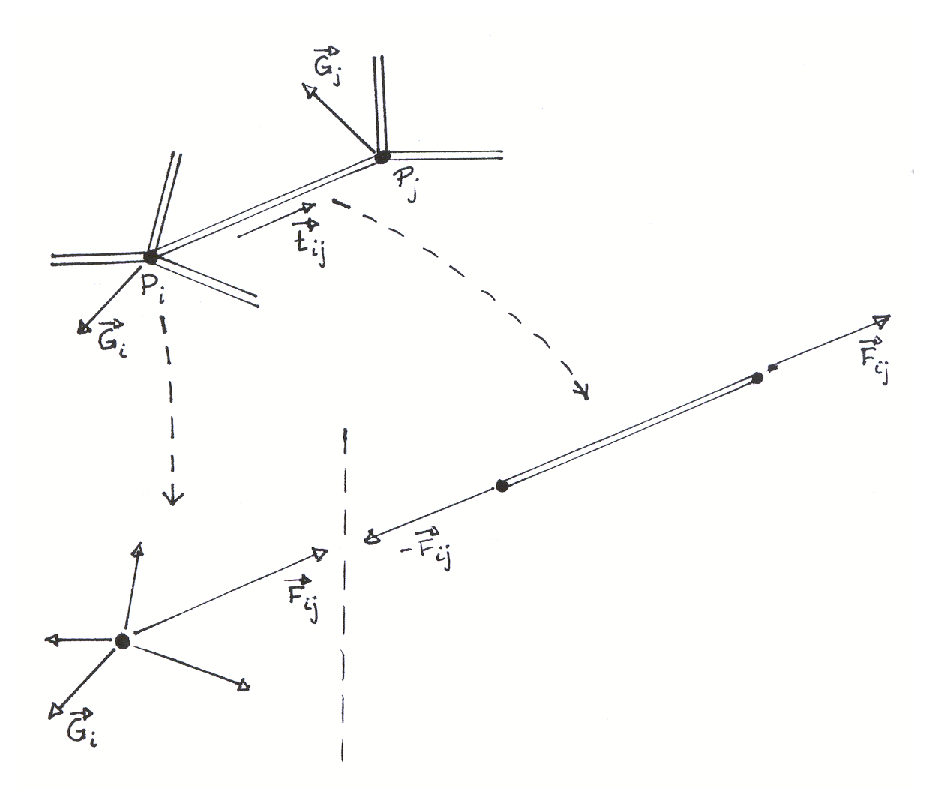
\epsfig{file=kuvat/kuvaM-2.ps}
\end{center}
\end{figure}
Kuvassa kuormitustilaa on purettu kahdeksi nk.\ \pain{va}p\pain{aaka}pp\pain{alekuvioksi}, 
joissa kummasakin vallitsee voimatasapaino. --- Huomattakoon, että liitoksia koskeva 
tasapainoehto \eqref{m-8.7} on hyvin samankaltainen kuin sähköpiirejä koskeva Kirchhoffin laki
\eqref{m-8.1}, joka myös on tasapainoehto (virtoja koskeva).

Kun yhtälöryhmässä \eqref{m-8.7} vektoriyhtälöt puretaan koordinaattimuotoon karteesisessa 
koordinaatistossa, niin skalaaristen yhtälöiden kokonaismääräksi tulee $2p$ tai $3p$ riippuen
siitä, onko kyseessä taso- vai avaruusristikkorakenne. Tuntemattomien $F_{ij}$ lukumäärä on 
luonnollisesti sama kuin sauvojen lukumäärä rakenteessa. Yhtälöryhmä \eqref{m-8.7} voi olla 
suoraan yksikäsitteisesti ratkeava, jolloin sanotaan, että rakenne on 
\pain{staattisesti} \pain{määrä}y\pain{t}y\pain{vä}. Tavallisempi tilanne on kuitenkin, että 
systeemi \eqref{m-8.7} on alimääräytyvä, eli \pain{staattisesti} \pain{määräämätön}. Tällöin 
tarvitaan tasapainolakien lisäksi toinen fysiikan laki,
\index{Hooken laki}%
\pain{Hooken} \pain{laki} 
(\hist{R. Hooke}, 1678). Hooken lain mukaan jokainen sauva käyttäytyy ristikkoa kuormitettaessa
kuten jousi, ts.\ voima $F_{ij}$ on suoraan verrannollinen sauvan \pain{ven}y\pain{mään}.

\mbox{\parbox{2in}{Oletetaan, että ristikkoa kuormitettaessa solmu $P_i$ 
(paikkavektori $\vec{r}_i$) siirtyy paikkaan $Q_i$, ja merkitään \pain{siirt}y\pain{mää} 
$\vec{u}_i = \Vect{P_i Q}_i$. Olettaen, että siirtymät ovat pieniä verrattuna sauvan pituuteen, 
voidaan kunkin sauvan venymä (negatiivinen venymä tarkoittaa puristumaa) laskea likimäärin 
kaavasta (vrt.\ kuvio)}}
\mbox{\parbox{4in}{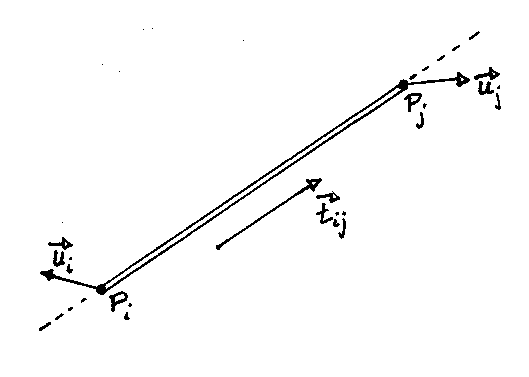
\epsfig{file=kuvat/kuvaM-3.ps}}}
\[
\abs{(\vec{r}_i + \vec{u}_i) - (\vec{r}_j + \vec{u}_j)}\ - \ \abs{\vec{r}_i - \vec{r}_j}\ 
                                     \approx\ (\vec{u}_j - \vec{u}_i) \cdot \vec{t}_{ij}.
\]

(Approksimaatiossa oletetaan, että siirtymien $\vec{u}_i$ ja $\vec{u}_j$ sauvaa vastaan 
kohtisuorat komponentit eivät vaikuta sauvan pituuteen.) Hooken lain mukaan venymä on suoraan
verrannollinen voimaan, eli
\begin{equation} \label{m-8.8}
F_{ij}\ =\ K_{ij} (\vec{u}_j - \vec{u}_i) \cdot \vec{t}_{ij},
\end{equation}
missä $K_{ij}$ on sauvalle ominainen kerroin (jousivakio). --- Huomattakon jälleen analogia 
sähköpiireihin: Siirtymät $\vec{u}_i$ vastaavat jännitteitä, voimat $F_{ij}$ virtoja, ja 
Hooken laki \eqref{m-8.8} vertautuu vastuksia koskevaan Ohmin lakiin. Jos sauvat ovat 
tasapaksuisia ja tehty homogeenisesta materiaalista, on jousivakio $K_{ij}$ suoraan 
verrannollinen sauvan poikkipinta-alaan ja kääntäen verrannollinen sauvan pituuteen. Jousivakio
riippuu myös materiaalin laadusta nk.\ \pain{kimmokertoimen} (materiaalivakio) kautta. 

Hooken lakia \eqref{m-8.8} käyttäen tulee yhtälöryhmästä \eqref{m-8.7} lineaarinen, 
tuntemattomina siirtymävektorien $\vec{u}_i$ koordinaatit. Tuntemattomien määrä on siis joko 
$2p$ (tasoristikko) tai $3p$ (avaruusristikko). Jotta yhtälöryhmästä saataisiin säännöllinen, on
ristikko vielä 'maadoitettava', eli tuettava riittävästi. Tuentaehdot voivat olla esim.\ muotoa 
$\vec{u}_k = \vec{0}$, jolloin solmun $P_k$ siirtyminen rakennetta kuormitettaessa on estetty.
Tällaisessa solmussa ei voimatasapainoehtoja tarvitse kirjoittaa, sillä tasapainosta huolehtivat
(tuntemattomat) tukivoimat, jotka vastaavat sähköpiirin maadoitusvirtoja. Tuentaehdoilla on 
yleisesti estettävä sellaiset siirtymätilat, jotka eivät aiheuta rakenteessa mitään kuormituksia
($F_{ij} = 0\ \forall\ i,j$). Erityisesti koko rakenteen liikkuminen jäykkänä kappaleena on 
matemaattisessa mallissa estettävä. Kun tällaiset riittävät (fysikaalisesti usein ilmeiset)
lisäehdot on asetettu, tulee yhtälöryhmästä \eqref{m-8.7}--\eqref{m-8.8} säännöllinen.
Siirtymät $\vec{u}_i$ voidaan tällöin ratkaista ensin, ja näiden avulla edelleen 
(fysikaalisesti ehkä kiinnostavammat) kuormitukset $F_{ij}$ Hooken laeista \eqref{m-8.8}.

\begin{Exa} \label{ristikko} \ \ 

\parbox{2in}{Oheisessa (taso)ristikossa on sauvoja kahta tyyppiä, jousivakiot $K_1$ ja $K_2$. 
Sauvoja on $7$ kpl ja yhtälöryhmässä \eqref{m-8.7} on $3 \times 2 = 6$ yhtälöä 
(tuetuissa solmuissa $A,\,B$ voimatasapainosta huolehtivat tukivoimat), joten rakenne on 
staattisesti määräämätön. Kun siirtymiä solmuissa $P_i$ merkitään}
\mbox{\parbox{4in}{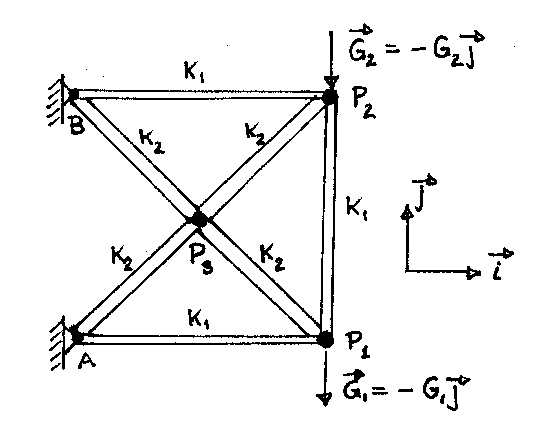
\epsfig{file=kuvat/kuvaM-4.ps}}}
\[
\vec{u}_i\ =\ u_i \vec{i} + v_i \vec{j}, \quad i = 1,2,3,
\]
niin lyhennysmerkinnöin
\[
a   = 1 + 2 K_2 / K_1, \quad b = 2 K_2 / K_1, \quad g_1 = G_1 / K_2, \quad g_2 = - G_2 / K_2
\]
yhtälöryhmä \eqref{m-8.7}--\eqref{m-8.8} saa muodon
\[ \left\{ \begin{array}{rrrrrrrrrrrrl} 
au_1&-&v_1& &    & &    &-& u_3&+& v_3&\quad 
                   = \quad&0\\ u_1&-&av_1& &    &+&bv_2&-& u_3&+& v_3&\quad = \quad&g_1\\
    & &   & &au_2&+& v_2&-& u_3&-& v_3&\quad 
                   = \quad&0\\    &-&bv_1&+& u_2&+&av_2&-& u_3&-& v_3&\quad = \quad&g_2\\
 u_1&-&v_1&+& u_2&+& v_2&-&4u_3& &    &\quad 
                   = \quad&0\\-u_1&+& v_1&+& u_2&+& v_2& &    &-&4v_3&\quad = \quad&0
\end{array} \right. \]

Tämä on säännöllinen ryhmä, josta siirtymät $u_i,\,v_i$ ovat ratkaistavissa. Sauvoja venyttävät
tai puristavat voimat ovat tämän jälkeen laskettavissa Hooken \mbox{laeista \eqref{m-8.8}.} 
Esimerkiksi sauvaa $P_1 P_3$ venyttää (negatiivisena puristaa) voima
\[
F_{13}\ =\ K_2\,[(u_3 - u_1)\vec{i} + (v_3 - v_1)\vec{j}\,] 
                          \cdot \frac{1}{\sqrt{2}}\,(-\vec{i}+\vec{j}) 
        = \frac{K_2}{\sqrt{2}}\,(u_1 - v_1 - u_3 + v_3). \loppu
\] 
\end{Exa}

\Harj
\begin{enumerate}

\item
Vastuspiirin solmut ovat tasasivuisen kolmion $ABC$ kärjet ja kolmion keskipiste $D$. Sivuilla
$AB$, $BC$ ja $CA$ on vastukset $R_1=1$, $R_2=2$ ja $R_3=3$. Kolmion kärjet $A$, $B$ ja $C$
on yhdistetty keskipisteeseen vastuksilla $R_4=R_5=2$ ja $R_6=3$. Olettaen virtasyöttö $I$
solmuun $A$ ja maadoitus solmuun $C$, muodosta lineaarinen yhtälöryhmä solmujen $A,B,D$ 
jännitteille ja laske solmujen $A$ ja $C$ välinen vastus.

\item
Kuution kärjet $P_i,\ i=0 \ldots 7$, on numeroitu siten, että $P_0$ ja $P_7$ ovat vastakkaiset
kärjet kuution yhdellä sivulla. Kärjet ovat solmuja virtapiirissä, jonka johdot kulkevat
pitkin kuution särmiä ja jokaisella särmällä vastus $=R$. Solmujen jännitteistä ($x_i$)
tiedetään, että $x_0=E$ (jännitelähde) ja $x_7=0$. Muodosta lineaarinen yhtälöryhmä
jännitteille $x_i,\ i=1 \ldots 6$. Ratkaise ja laske solmujen $P_0$ ja $P_7$ välinen vastus.

\item (*) \index{zzb@\nim!Silta}
(Silta) Tason ristikkorakenteen solmut $P_1,\ldots,P_7$ ovat pisteissä $(0,0)$, $(1,1)$,
$(2,0)$, $(3,1)$, $(4,0)$, $(5,1)$ ja $(6,0)$. Solmut on yhdistetty sauvoilla siten, että
muodostuu viisi vierekkäistä tasakylkistä ja suorakulmaista kolmiota. Solmu $P_1$ on jäykästi
tuettu ja solmun $P_7$ siirtyminen suuntaan $\vec j$ on estetty, muita tukia ei ole. Solmuihin
$P_3$ ja $P_5$ vaikuttavat kuormat ovat $\vec F_3=-a G\vec j$ ja $\vec F_5=-bG\vec j$, missä
$a,b \ge 0$ ovat dimensiottomia vakioita. Muita kuormia ei ole. Merkitse sauvoja
venyttäviä (negatiivisena puristavia) voimia symboleilla $T_i=x_iG$ ($11$ sauvaa!) ja kirjoita
näiden avulla solmujen tasapainoyhtälöt. Ratkaise systeemi (mahdollista, koska rakenne on
staattisesti määräytyvä), ja vastaa ratkaisun perusteella kysymykseen: Jos jokainen sauva
kestää puristusta $G$:n verran ja vetoa rajattomasti, niin millaiset kuormat ovat mahdollisia
rakenteen romahtamatta? Piirrä kuva $ab$-tasoon!

\end{enumerate}